
\documentclass[a4paper,12pt]{article}

\usepackage[T1]{fontenc}
\usepackage[utf8]{inputenc}
\usepackage[english]{babel}
\usepackage{graphicx}
\usepackage{xcolor}

\usepackage[backend=biber]{biblatex}
\addbibresource{bibliography.bib}

\renewcommand\familydefault{\sfdefault}
\usepackage{tgheros}
\usepackage{csquotes}
\usepackage[defaultmono]{droidmono}

\usepackage{amsmath,amssymb,amsthm,textcomp}
\usepackage{enumerate}
\usepackage{multicol}
\usepackage{tikz}

\usepackage{float}
\restylefloat{figure}
\restylefloat{table}

\usepackage{geometry}
\geometry{total={210mm,297mm},
left=25mm,right=25mm,%
bindingoffset=0mm, top=20mm,bottom=20mm}
\linespread{1.5}

% my own titles
\makeatletter
\renewcommand{\maketitle}{
\begin{center}
\vspace{2ex}
{\normalfont \textsc{\@title}}
\vspace{1ex}
\\
\rule{\linewidth}{0.5pt}
\\
\@author \hfill \@date
\vspace{2ex}
\end{center}
}
\makeatother
%%%

% custom footers and headers
\usepackage{fancyhdr}
\pagestyle{fancy}
\lhead{}
\chead{}
\rhead{}
\lfoot{}
\cfoot{}
\rfoot{\thepage}
\renewcommand{\headrulewidth}{0pt}
\renewcommand{\footrulewidth}{0pt}
%

%%%----------%%%----------%%%----------%%%----------%%%

\begin{document}

\title{MS715 - Production Planning and Control}

\author{Gabriel Stefanini}

\date{\today}

\maketitle

\begin{abstract}
   A long line of scientific endeavour addresses problems in the 
   manufacturing and agriculture decision-making cycles. The scope of the course comprises the role of planning and control in the context of production of a good or a set of goods. Evaluating whether a production work-flow is effective or not and looking into the future and making forecasts is a very complex task for humans beings.
   
   Operations Research techniques contribute to making setting up a production and scheduling plan a more elucidated and mathematically-reasoned decision. In this summary, we had a hands-on experience working with real-world data and statistical models and the opportunity to implement and carry out tests regarding different demand and inventory scenarios and examine the corresponding best obtainable solution. 
\end{abstract}

\section{Article Summary}
    The assigned article for reviewing is part of master thesis from an Icelandic engineer from Reykjavík University, submitted to the School of Science and Engineering 
    under the title "Linear Optimization model that maximizes the value of pork products" \cite{reynisdottir}. 
    
    The author constructs and investigates a linear programming mathematical model for the production chain of pork at one of Iceland's biggest slaughterhouses. Food processing is the most important export industries in Iceland, corresponding to 36.1\% of total numbers of companies.
    
    Among the industries of this sector, fishing is the main activity and has taken advantage of optimization-based solutions for many years. The article proposes to extend these benefits to other industries, such as meat processing,  therefore achieving better utilization of production and increasing the profitability.
 
    At first, the food processing is a multi-phase industry. It  incorporates many factors and activities, making identifying bottlenecks and predicting failures nearly impossible. Below we see simplified work-flow of the processes involved in pork production.
    
\begin{figure}[H]
\centering
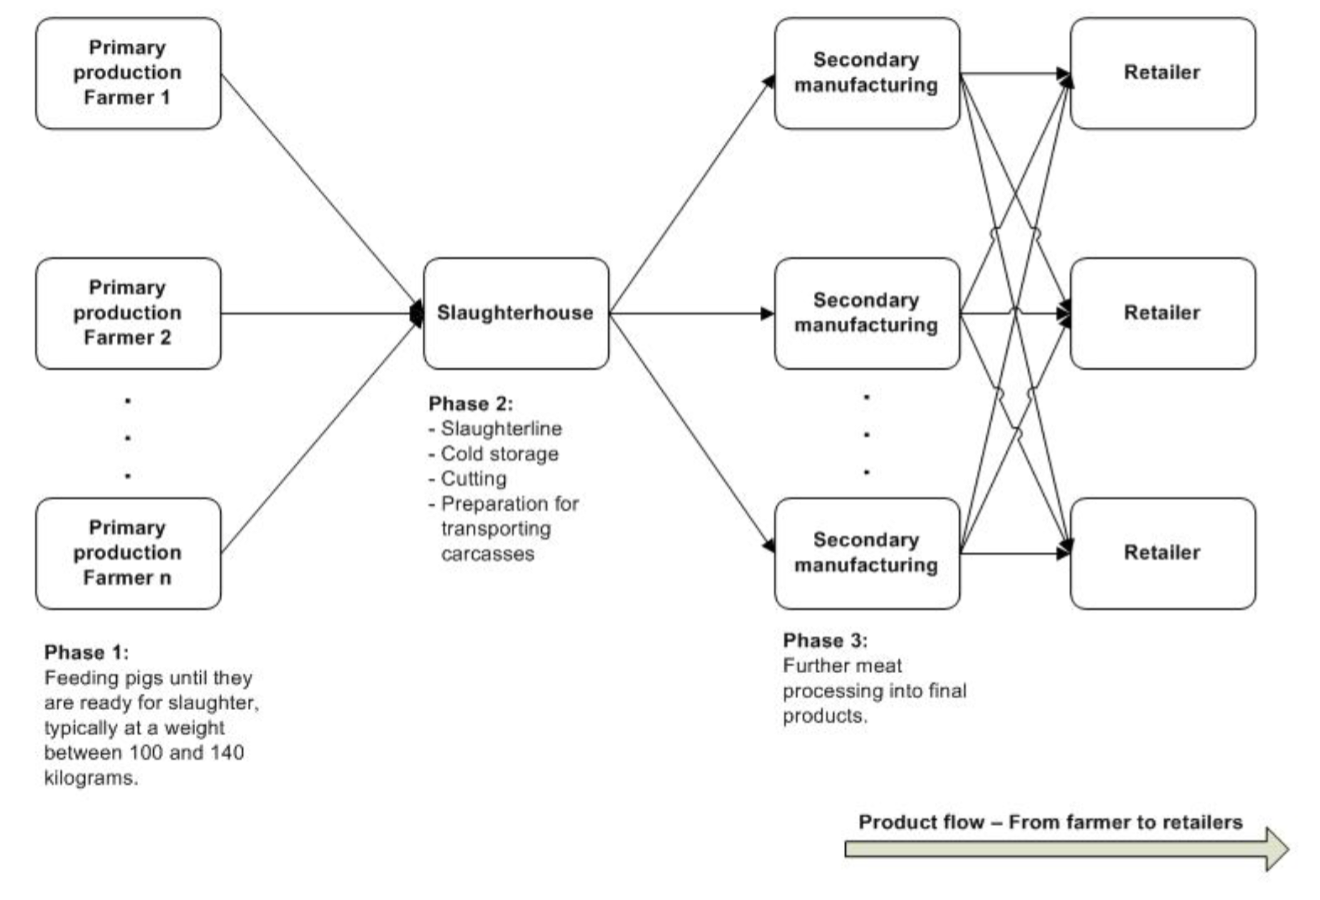
\includegraphics[width=0.5\textwidth]{1.png}
\caption{Food processing phrases}
\end{figure}

    At phase 2 is where the decision-making model shows its value. Linear programming and optimizing for a global objective function guarantees profitability in spite of limitations and even regarding co-production. Co-production consists in a process in which manufacturing a main product requires manufacturing alongside a different product. In comparison, a by-product is usually an undesirable product.
    
    Regarding the pork production, decision-making steps were divided into three levels. For each production, there is a work-flow suck as the one illustrated below.
    
\begin{figure}[H]
\centering
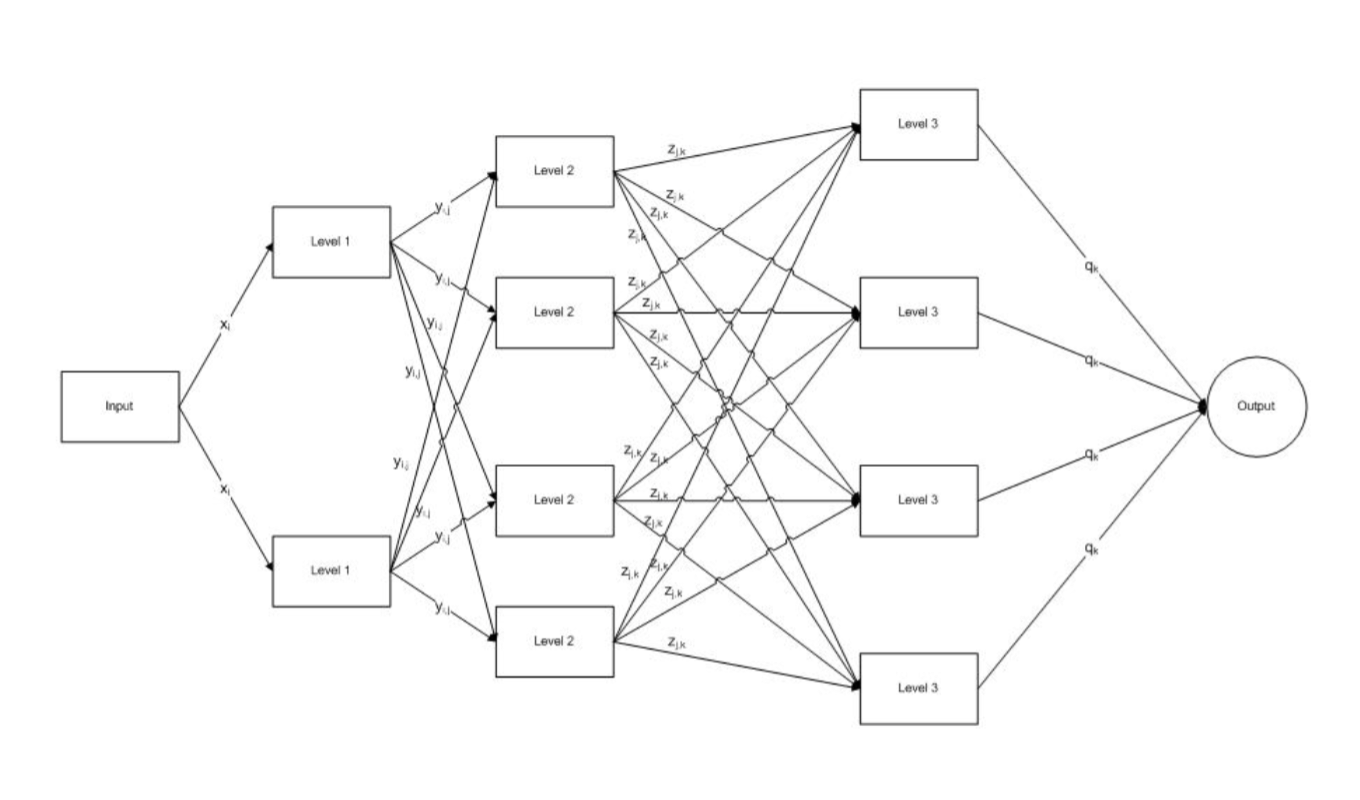
\includegraphics[width=0.5\textwidth]{2.png}
\caption{Production levels}
\end{figure}
    
     The model demonstrated good results comparing to the real-world. Even a simplified mathematical model such as a linear programming one considering many premises and approximations could support the decision-making process and maximize revenues.
    
It contributes to clarifying and assuring production plans in the food industry and can as well as be extended to other areas. The article proved
    that systematically establishing a planning culture within an organizing can contribute to visibility, profitability and better decisions. 
    
\section{Related Concepts}

The keys concepts are shared between the assigned article and the final project of the course.

\begin{itemize}
    \item Forecasting
    \item Inventory Control
    \item Production Planning
    \item Linear Programming
\end{itemize}

\section{Project}

The final project also approaches the decision-making task with a very similar linear programming model. However, some compromises have been made comparing to the article.

\begin{itemize}
    \item Data \\
        Most of the research effort demonstrated on the article was collecting and making sense out of the data. The final project project adopted a more simplified model and took advantage of existing data.
    \item  Cross validation \\
        We could not compare the results to the real production plans.
    \item Inventory Control \\
        At some extent, the article addresses how inventory could impact profitability whereas the final project focuses on the model's feasibility. 
    \item Sensibility Analysis \\
        Although the final project shows results for different parameters and demand scenarios, it lacks a deeper and mathematical-proven sensibility analysis.
\end{itemize}

\section{Mathematical model}

The mathematical approach to the decision-making challenge is a linear programming model. In this class of optimization techniques, the objective function and all inequalities relating to some condition are linear. In 1947, the american mathematican George Dantzig published his Simplex algorithm which solves deterministically and in polynomial time this type of problem. In effect, it is listed as one of the top 10 algorithms of the twentieth century. Modern solvers, such as CPLEX \cite{cplex} and Gurobi \cite{gurobi}, achieve results fairly quickly.

The present model was implemented using AIMMS \cite{aimms}. In 1993, AIMMS was introduced as a new type of algebraic modeling language (AMP). It consists of an integrated combination of a modeling language, a graphical user interface, and numerical solvers.\\

The mathematical was constructed as follows. 

\begin{table}[H]
\centering
\begin{tabular}{|c|c|}
\hline
\textbf{Indices} & \textbf{Definition} \\
\hline 
 $i$ & Division of the carcass \\
\hline
 $j$  & Intermediary raw material \\
\hline
 $k$  & Product \\
 \hline
 $t$  & Planning horizon \\
 \hline
\end{tabular}
\caption{Indices}
\label{tab:indices}
\end{table}

\begin{table}[H]
\centering
\begin{tabular}{|c|c|c|}
\hline
\textbf{Parameters} & \textbf{Unit} & \textbf{Definition} \\
 \hline
 $input_t$ & Kg & Weight of total carcass to process in time period $t$  \\
 \hline
 $part_i$ & \% & Proportion of division $i$ $k$  \\
\hline 
 $val_k$ & \$ & Value of product $k$  \\
\hline 
 $dem_{t, k}$ & \$ & Demand of product $k$ in time period $t$  \\
\hline
 $\alpha_{j, k}$ & \% & Lower limit of product $k$ from a raw material $j$ \\
\hline 
 $\beta_{j, k}$ & \% & Upper limit of product $k$ from a raw material $j$ \\
\hline 
 $c_1$ & \$ & Vendor cost at level 1 \\
\hline
 $c_3$ & \$ & Vendor cost at level 3 \\
\hline
 $ic$  & \$ & Inventory cost \\
 \hline
 $dp$  & \% & Production deterioration \\
 \hline
\end{tabular}
\caption{Parameters}
\label{tab:parameters}
\end{table}

\begin{table}[H]
\centering
\begin{tabular}{|c|c|c|}
\hline
\textbf{Decision Variables} & \textbf{Unit} & \textbf{Definition} \\
\hline 
 $\chi_{t, i}$    & Kg & Amount of division $i$ in time period $t$ \\
\hline
 $\psi_{t,i,j}$   & Kg & Amount of raw material $j$ from division $i$ in time period $t$ \\
\hline
 $\omega_{t,j,k}$ & Kg & Amount of product $k$ from raw material $k$ in time period $t$ \\
\hline
 $prod_{t, k}$    & Kg & Production of product $k$ in time period $t$ \\
\hline
 $inv_{t, k}$     & Kg & Inventory level of product $k$ in time period $t$ \\
\hline
 $level1_{t, i}$  & Kg & Amount of extra material in time period $t$ \\
\hline
 $level3_{t, k}$  & Kg & Amount of extra material in time period $t$ \\
\hline
\end{tabular}
\caption{Decision variables}
\label{tab:decision_variables}
\end{table}

\begin{itemize}
    \item \textbf{Objetive Function}
        \begin{equation}
            \max z = \sum_{t \in T}\sum_{k \in K}\sum_{i \in I} (P_{t, k} - I_{t, k} -V_{t, i} - U_{t, i}) - \sum_{k \in K} {D_k}
        \end{equation}
    
        \begin{itemize}
            \item Production Profit \\ 
                $P_{t, k} = val_k \cdot prod_{t, k}$
            \item Inventory Cost  \\
                $I_{t, k} = ic \cdot inv_{t, k}$
            \item Vendor Cost      \\
                $V_{t, i} = c_1 \cdot level1_{t, i}$ \\
                $U_{t, k} = c_3 \cdot level3_{t, k}$ 
            \item Deterioration Cost \\
                $D_{k} = val_k \cdot inv_{t_{last}, k} \cdot dp$ 
        \end{itemize}
    \item \textbf{Constraints for first level production}
        \begin{equation}
            \chi_{t, i} = part_i \cdot input_t + level1_{t, i} \qquad \forall{t, i}
        \end{equation}
    \item \textbf{Constraints for second level production}
        \begin{equation}
            \sum_{j \in J} \psi_{t, i, j} = \chi_{t, i} \; \qquad \forall{t, i}
        \end{equation}
    \item \textbf{Constraints for third level production}
        \begin{align}
             \sum_{j \in J} \psi_{t, i, j} &= \chi_{t, i} \quad \qquad \forall{t, i} \\
             \sum_{k \in K} \omega_{t, j, k} &= \sum_{i \in I} \psi_{t, i, j} \quad \forall{t, j} \\
        \end{align} 
    \item \textbf{Constraints for production limits}
        \begin{align}
            \omega_{t, j, k} &\geq \alpha_{j, k} \cdot \sum_{i \in I} \psi_{t, i j} \quad \forall{t, j, k} \\
            \omega_{t, j, k} &\leq \beta_{j, k} \cdot \sum_{i \in I} \psi_{t, i j} \quad \forall{t, j, k}
        \end{align}
        
    \item \textbf{Constraints for production balance}
        \begin{equation}
            prod_{t, k} = \sum_{j \in J} \omega_{t, j, k} 
            \quad \forall{t, k}
        \end{equation}    
    \item \textbf{Constraints for inventory balance}
        \begin{align}
            inv_{t, k} &= prod_{t, k} - dem_{t, k} + slack_k 
            \quad \;\; \forall_{t=1, k} \\
            inv_{t, k} &= inv_{t-1, k} + prod_{t, k} - dem_k
            \quad \forall_{t>1, k}
        \end{align}
\end{itemize}

Furthermore, in order to evaluate the forecast and costs impact, 
we performed a parametric plot of the objective function changing one of the parameters. It consists in an empirically method for evaluating the sensibility analysis. 

\begin{figure}[H]
\centering
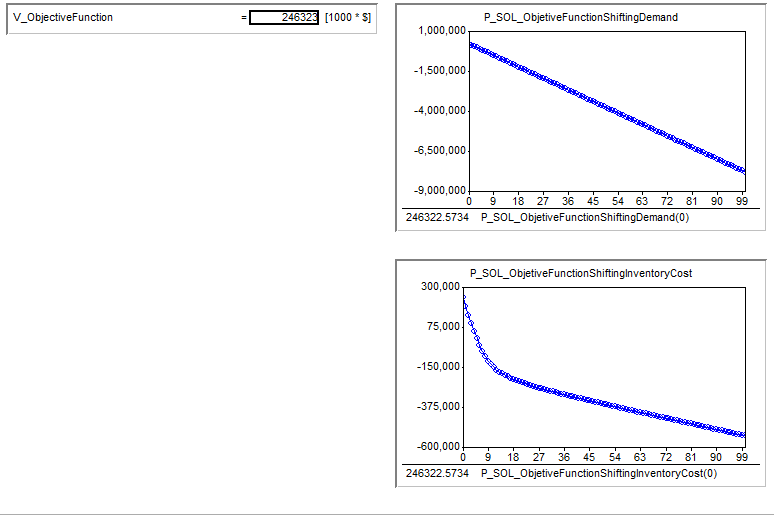
\includegraphics[width=0.5\textwidth]{3.png}
\caption{Objective function with constant demand along horizon}
\end{figure}

The demand and costs parameters were fixed at a constant value, which yields the official result for the scenario. After, we investigated how increasing these parameters impacted on the objective function. As we can see above, increasing the demand lin- early makes the objective function linearly smaller whereas increasing the inventory cost has a more particular effect.

\begin{figure}[H]
\centering
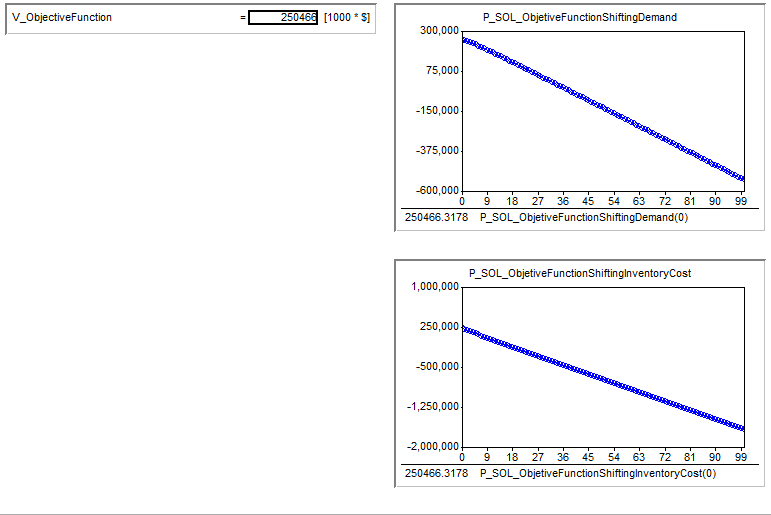
\includegraphics[width=0.5\textwidth]{4.png}
\caption{Objective function with increasing demand linearly along horizon}
\end{figure} 

Operations Research methods and mathematical modeling have contributed for many years with creating production plans in the food industry and other diverse appli- cations. The article proved that systematically establishing a planning culture within an organization leads to visibility, profitability and better decisions.


\printbibliography

\end{document}